\section{The Compact Muon Solenoid}
At one of the collision points of the LHC, the CMS detector\cite{CMS, Bayatian:2006zz} is placed. Weighing 14 000 \si{ \tonne}, This cylindrical detector is about 28.7 \si{ \meter} long and 15 \si{ \meter} in diameter, weighing around 14 000 \si{ \tonne}. It has an onion like structure of several specialised detectors and contains a superconducting solenoid with a magnetic field of 3.8 \si{ \Tesla}. The CMS detector is designed in a way that it can address the needs of physics coming from the LHC. Living in a hadronic environment, multi-jet processes produced by the strong interaction are a main source of background for rare physics processes. Therefore, good identification, momentum resolution, and charge determination of muon, electrons and photons is one of the main goals of the CMS detector. Further it provides a good charged particle momentum resolution and reconstruction efficiency in the inner tracker such that for example jets coming from b quarks or tau particles can be identified. Also th electromagnetic resolution for an efficient photon and lepton isolation as well as a good hadronic calorimeter for the missing transverse energy were kept into account while designing CMS. 

The LHC provides many collisions in a short amount of time. In order to discriminate between consecutive collisions - known as out of time pile up events - , CMS has to complete the full data acquisition for one collision event before the next one happen (around 50 \si{ \nano \second} (FIXME) ). Furthermore, since the photons are in packets, around 21 (FIXME) inelastic collisions happen every beam crossing. This creates a great amount of background processes in the detector called in time pile up events. Due to this difficult conditions, the detector has a great granularity which on its turn creates a need for huge number of synchronized electronic channels. Furthermore, due to to high flux of particles in the regions close to the beam, the electronics has to be able to endure high radiation. 

\subsection{CMS coordinate system}
The coordinate system used by CMS can be found in Figure~\ref{fig:CMScoord}. The origin of the right handed orthogonal coordinate system is chosen to be the point of collisions. The x-axis points towards the centre of the LHC ring such that the y-axis points towards the sky, and the z-axis lies tangent to the beam axis. Since the experiment has a cylindrical shape, customary coordinates are used to describe the momentum \impuls: the distance $\rho$, the azimuthal angle $\phi \in \left[-\pi,\pi\right]$ - the angle between the x-axis and the projection in the transverse plane of \impuls (\trimpuls) - , the pseudo-rapidity \psrap - expressed by the polar angle $\theta$ between the direction of \impuls and the beam - : 
\begin{equation}
\eta = - \ln \left(\tan \left(\frac{\theta}{2}\right)\right).
\end{equation}
For the energies considered at the LHC, where $E >> m$, the pseudo-rapidity is a good approximation of the rapidity $y$
\begin{equation}
y = \frac{1}{2} \ln \left(\frac{E + p_z}{E - p_z}\right), 
\end{equation}
where the difference of rapidities of two particles is invariant under a Lorentz boost in the z-direction.
 \begin{figure}[ht]
	\centering
	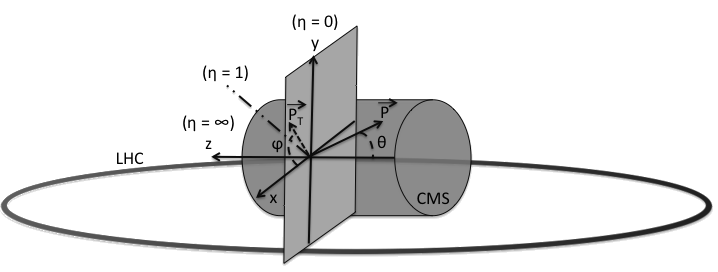
\includegraphics[width=0.75\textwidth]{2_ExperimentalSetup/Figures/imageedit_1_9146672677}
	\caption{Representation of the coordinate system used by CMS. The point of origin is put at the collision point. The x-axis points towards the centre of the LHC ring such that the z-axis lies tangent to the beam axis. }
	\label{fig:CMScoord}
\end{figure}

\subsection{Towards the heart of CMS}
The CMS consists of two parts; a central barrel around the beam pipe (\abspsrap $<1.4$) and two plugs to ensure the hermeticity of the detector. In Figure~\ref{fig:CMS} the onion like structure of the CMS detector is visible. The solenoid contains the hadronic calorimeter,  the electromagnetic calorimeter and the tracker, while the muon chambers are placed outside the solenoid.


\begin{figure}[ht]
   \centering
	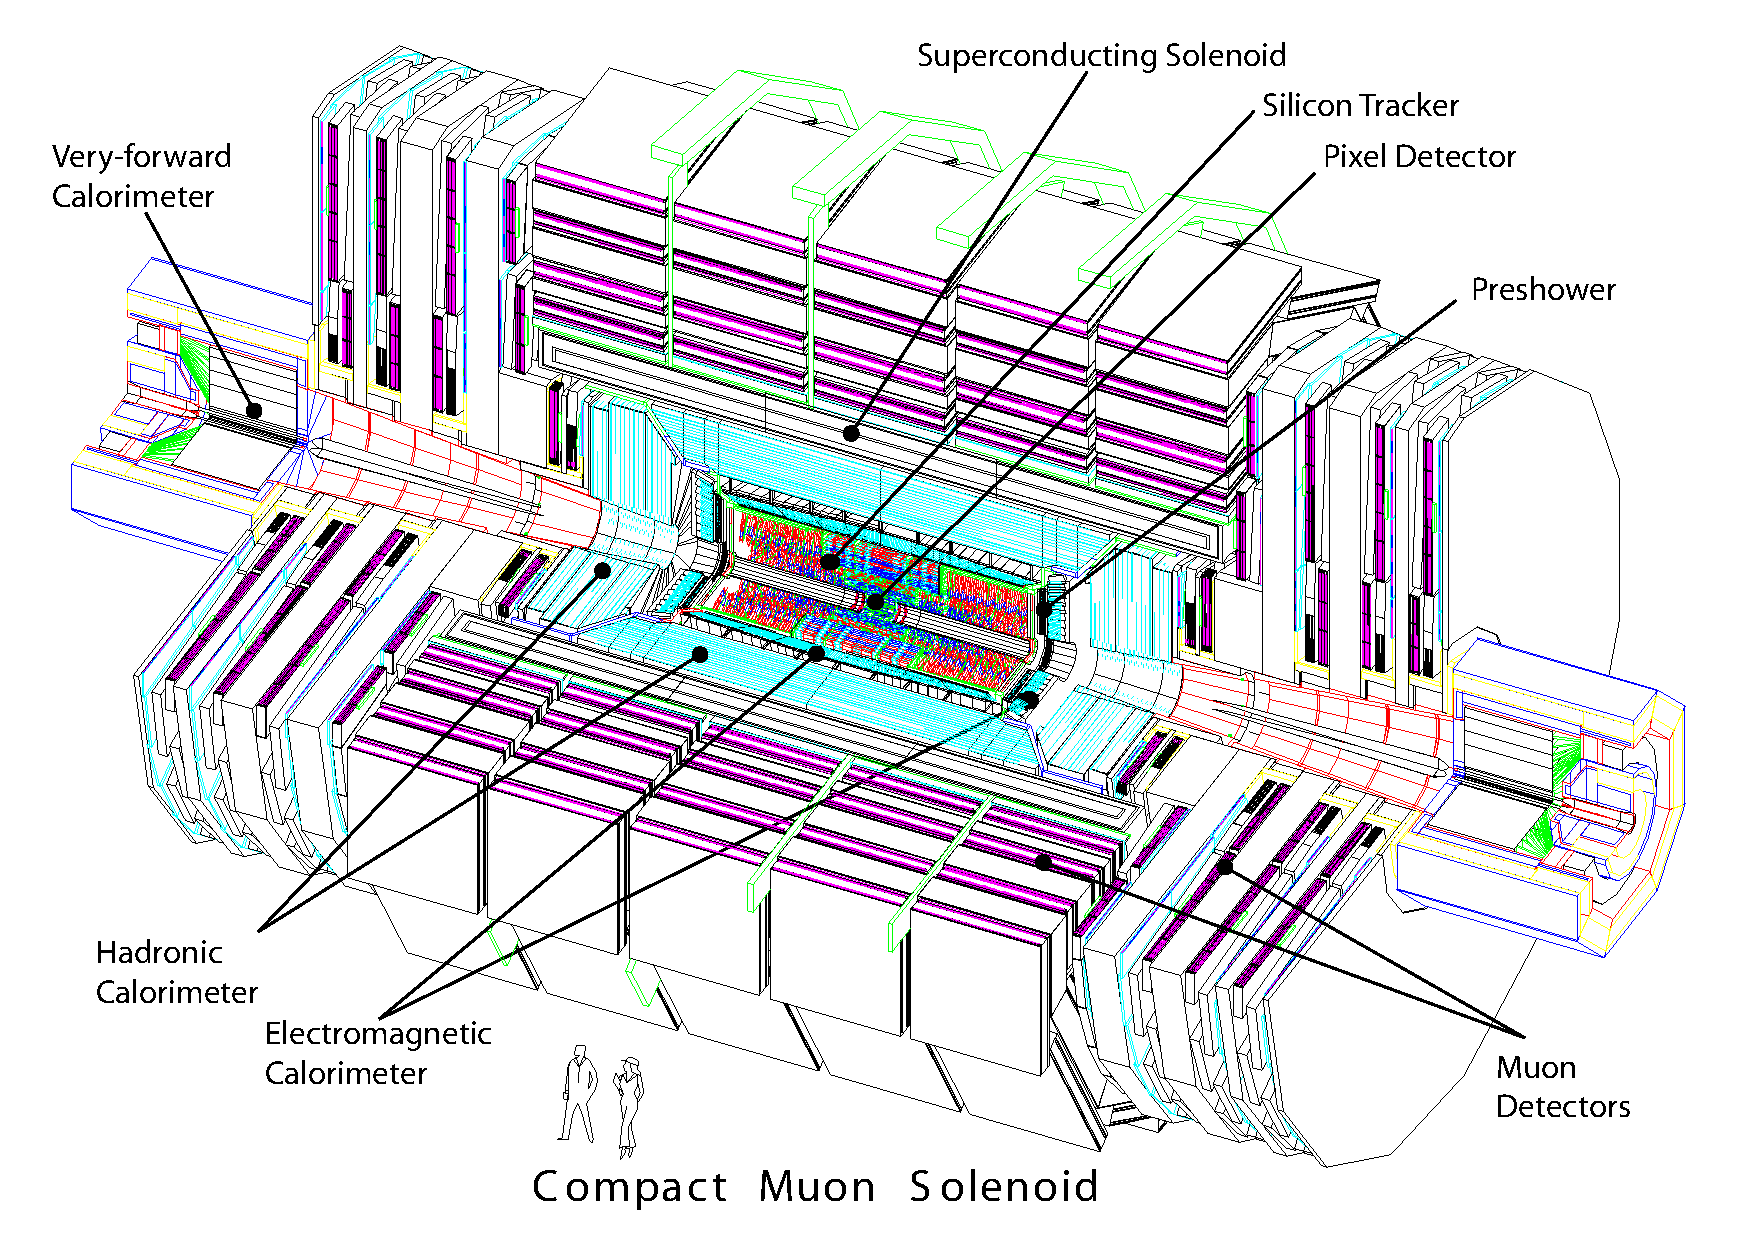
\includegraphics[width=\textwidth]{2_ExperimentalSetup/Figures/cms_complete_labelled}
	\caption{Mechanical layout of the CMS detector\cite{CMSdraw} (FIXME)
		.}
	\label{fig:CMS}
\end{figure}
	

\subsubsection{Inner tracking system and operations}
%https://indico.cern.ch/event/632928/
\subsubsection{Electromagnetic calorimeter}
\subsubsection{Hadronic calorimeter}
\subsubsection{Muon system}

\subsection{Data acquisition}
\subsection{CMS computing model}
%CMS trigger system 
% https://arxiv.org/abs/1609.02366